\normallinespacing

%\chapter{Introduction}

% Goals of the thesis etc. 
% Stress that the goal is to create a useful tool, combining phonemes and prosody

\normallinespacing

\chapter{Introduction}

Compared to written language, speech is a complex, multi-faceted dimensional signal. Linguistic analysis distinguishes between two primary components: the phonetic segments or phonemes on the one hand, and prosodic features like pitch movements, amplitudes, and duration on the other. Standard orthographies of written language capture mostly only the phonemic part of speech, which can be reduced to discrete elements that are represented by letters, or graphemes. To be sure, written language has developed its special devices, such as headings, paragraphs, or bullet lists. But compared to the human voice, orthographic representation of text is "flat", hardly able to capture the expressive dimension of language \cite{pataca2021speech}. This straight-jacket is felt in current digital communication, where users frequently attempt to get rid of these limitations by additional symbols, like emojis \cite{zappavigna2024}, but also by non-standard orthography, using "visual prosody" like all-caps to signal prosodic highlighting, emotive arousal, or additional iconic meanings, such as by vowel elongation (e.g., \textit{booooring}) to mimic intonational lengthening \cite{fuchs2019}, \cite{heath2020no}. 

With the advent of text-to-speech and speech-to-text systems, the gap between speech and writing has narrowed dramatically. However, automated speech recognition (ASR) prioritizes orthographic transcription over fine-grained acoustic data, as represented, e.g., by the International Phonetic Alphabet (IPA) \cite{internationalphoneticassociation1999ipa}. This creates a gap between the richly expressive nature of the human voice and the simplified representation provided by standard orthography. It may be the optimal way to go for applications like dictation devices for business applications, but it may be suboptimal, for example, for subtitle generation for movies. 

In this thesis, we will conceive, and partially develop, a tool, called SpeechPrint, which enables the integration of prosodic features in the written representation of spoken language. The range of applications of such a tool is considerable -- from lively representations of subtitles over the voice input to create more expressive chats to the visualizations of recitations of poems. We will discuss such possible uses, but for the purpose of this thesis we will focus on the specific task to create a symbolic representation of prosodic features that is able to support such uses. To be specific, we will develop a tool that assists in the transcription of speech for purposes of linguistic research. This rather specific use scenario helps us to focus on the extraction of relevant prosodic features, in particular lengthening, pitch movement, and amplitude. We think that it should also be a useful device fields like conversation analysis and field work on under-resourced languages. 

There are excellent tools available to visualize and study speech. One, Praat, was initiated more than 20 years ago and continuously developed, and is now used all over the world in linguistic and phonetic labs, but also for the study of animal communication. But with the advent of ASR, there are increasingly capable tools that assist in the transcription and annotation of speech. They have to be trained for the languages that they are used for, and this means, they are better in large, wide-spread languages of economic importance than in smaller languages with fewer resources. However, they typically have the goal of standard orthographic representations that are time-aligned on the level of utterances. Programs that time-align speech segments like phonemes are rarer, and those that also attempt to render prosodic features are highly specialized. 

Our goal is to investigate and test available modules with this more specialized orientation, and bundle them together to one device that provides time-aligned phonemes and a prosodic representation. The immediate goal was to create a tool that should be of help for linguists that are not specialized in phonetic research, such as conversation analysis \cite{hutchby2008} and linguistic field work \cite{thieberger2012}, \cite{rozhanskiy2021}. SpeechPrint, at the planned stage, should provide a pre-transcription analysis with phonemes and time-aligned syllables, and a symbolic representation of pitch and amplitude matched to the syllables. This pre-analysis can be used as a help for a more precise, human-guided transcription effort. The result can be only as good as the current tools that we found in the current stage of development. It is not surprising that they are better with large languages like English and Spanish than with smaller languages. 

The thesis proceeds as follows. In Chapter \ref{StateOfArt}, we will give a very brief sketch of the current state of spoken language research, as far as it is relevant for this thesis. It focuses on phonemes and prosody, and introduces two main tools, Praat and ELAN. In Chapter \ref{ASR} we will discuss Automated Speech Recognition and important recent tools that have been developed from this research, in particular phoneme aligners and prosody analyzers. Chapter \ref{speechprint} is devoted to the description of the tool SpeechPrint, and in Chapter \ref{testing} we will put it to various tests. The final chapter, \ref{scenarios}, consists in a discussion of what is achieved, of what remains to be achieved, and in particular, of some usage scenarios of representing prosodic features typographically, or more general, graphically, to bring alive the vividness and expressiveness of speech in the visual domain. 



% In mediated spaces, if the digital profile is the costume, then typography is the voice \cite{sasamoto2015relevance}. However, the manual manipulation of text to represent prosody is often impressionistic and lacks a systematic link to acoustic reality \cite{pataca2021speech}. Current research in multimodal stylistics suggests that typographical features like font-weight and baseline shift can serve as effective visual proxies for magnitude (loudness) and pitch ($F_0$) \cite{pataca2021speech}, \cite{sasamoto2015relevance}. Yet, the labor required to manually synchronize these visual cues with spoken audio remains a significant barrier for researchers and creators alike.

% The primary objective of this thesis is to bridge this gap by developing \textbf{SpeechPrint} (also referred to as the \textbf{EmEt} tool), a computational framework designed to be a useful and accessible tool for researchers \cite{dryer2013wals}, \cite{maddieson2013consonant}. The central goal is to create a system that combines the identification of categorical phonemes with the extraction of quantitative prosody, such as pitch trajectories, duration, and amplitude \cite{maddieson2013vowel}, \cite{kuhl2004early}. By adopting an "EmEt" (emic/etic) philosophy, SpeechPrint transforms human speech into a representation that preserves the "phonetic fingerprint" of the speaker while allowing for automated, reproducible annotation \cite{pataca2021speech}, \cite{clement2013sounding}.

% By integrating these layers, the thesis aims to support diverse usage scenarios, ranging from the scientific analysis of endangered languages in the DoReCo project to the aesthetic visualization of sound structures in recited poetry \cite{chomsky1968sound}, \cite{mccurdy2016poemage}. For literary scholars, SpeechPrint facilitates a "literacoustic" reading of texts, allowing for the visualization of a poem's "sonic topology"—the complex interactions of rhyme, rhythm, and pitch that interact across the spatial field of the text \cite{mccurdy2016poemage}, \cite{clement2013sounding}. Ultimately, this work treats speech as "Dynamic Vector Graphics," where temporally aligned phonetic units become navigable objects for both scientific inquiry and artistic expression \cite{pataca2021speech}.

\chapter{The Multidimensional Signal: Layers of Meaning in Spoken Language}
\label{StateOfArt}

The purpose of this chapter is to introduce the reader to basic aspects of speech research, the investigation of spoken language. This is, of course, a very wide field covering linguistic, cognitive, and physiological aspects. We will concentrate strictly on the topics that are relevant for my own proposal: The segmental phonemes and supra-segmental prosodic units of language, and two very popular research tools, Praat and Elan. 

\section{Elements of spoken language}

In this section we will first discuss phonemes in spoken language and then turn to prosodic features, which are easily underrated in their importance. 

\subsection{Segments: The building blocks of meaningful units}

One essential characteristic of human languages is what has been called "duality of patterning" or "double articulation" \cite{hockett1958course}, \cite{martinet1960elements}: The smallest meaningful units of human speech, such as individual words, consist of sequences of units that themselves have no meaning—the speech sounds or phonemes \cite{hockett1958course}. For example, the English word \textit{dogs}, consisting of the lexeme \textit{dog} and the suffix morpheme \textit{-s}, is expressed by the sequence of phonemes that can be rendered as /\textipa{dO:gz}/, according to the International Phonetic Alphabet (IPA) \cite{internationalphoneticassociation1999ipa}. 

Phonemes can be realized differently by different speakers and in different contexts. They can be realized by different "allophones", such as English /p/ as aspirated in [\textipa{p\super{h}In}] \textit{pin} and non-aspirated in [\textipa{spIn}] \textit{spin}, but more importantly they often have a range of realizations \cite{internationalphoneticassociation1999ipa}. For example, the velar stop /k/ is realized more fronted in \textit{kit} than in \textit{cat}. This range of possible realizations is most dramatic with vowels, not only between speakers but also for a single speaker. For example, in a study that investigated both the physiology of production and the acoustic features of vowels, the spread of vowels, characterized by their first and second formants $F_1$ and $F_2$ as illustrated in Figure~\ref{fig:vowelvariation}, was reported. Note the considerable amount of overlap in this reduction of continuous values to discrete categories, which is mostly due to the influence of adjacent phonemes that affect the realization, a phenomenon known as "coarticulation" .

\begin{figure}
    \centering
    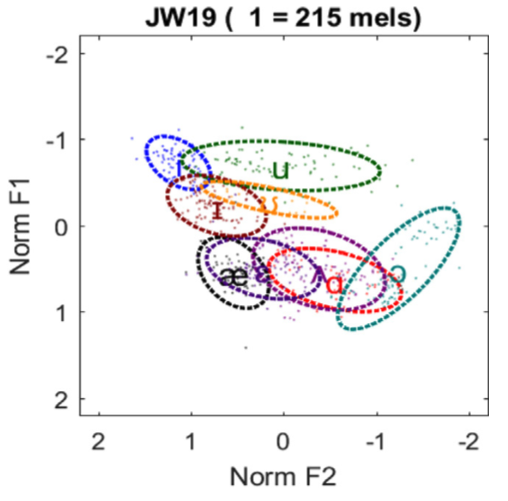
\includegraphics[width=0.5\linewidth]{vowelvariation.png}
    \caption{Realization of vowels by an English speaker, adapted from \cite{whalen2018}.}
    \label{fig:vowelvariation}
\end{figure}

It is remarkable that each language makes use of a small set of phonemes to express a much wider variety of lexical meanings. This set is in the magnitude of about 25 consonants and 8 vowels on average, but shows a considerable variation (e.g. from 6 consonants in the Oceanic language Rotokoas and 122 consonants in the San language !Taa, \cite{dryer2013wals,maddieson2013consonant,maddieson2013vowel}). These phonemes distinguish between different meanings (e.g.\ /\textipa{dO:gz}/ vs.\ /\textipa{lO:gz}/ and /\textipa{di:gz}/) and are acquired by children during their first year, before other aspects of language learning develop \cite{kuhl2004early}. The phonemic structure is the ultimate reason why alphabetic writing is possible: The letters, or graphemes, and their order on the page correspond in some tighter or looser way to the phonemes and their order in time. 

\subsection{Suprasegmentals: Prosody}

However, in addition to the digital and sequential nature of phonemes, often called "segments", spoken language is also characterized by prosody. Prosodic features typically apply to sequences of segments, like syllables, words, syntactic phrases, or whole speech acts, and hence are called "supra-segmentals". They also contribute to meaning. Famously, in tone languages like Mandarin or Yoruba, they distinguish between different lexemes or grammatical meanings. For example, Mandarin \textit{b\=eizi} 杯子 means `cup, glass', whereas \textit{b\`eizi} 被子 means `quilt, blanket', where the macron (\={}) and grave accent (\`{}) denote high and falling pitch on the first syllable, respectively. In Edo, a West-African languages, pitch can distinguish grammatical meanings, as in \textit{ì mà} ‘I show’ (present, habitual), ì má ‘I showed’ (past tense) and \textit{í mà} ‘I am showing’ (progressive) \cite{ladefoged1975}. But as we will see below, pitch variations are also used in languages like English for tasks like highlighting new or important parts of the message or backgrounding known of given parts, for distinguishing between speech acts like assertions, questions, exclamations, and callings, and for the expression of attitudes and emotions. As newer research shows, this often happens in combination with manual and facial gestures. 

The smallest unit in terms of sequences of phonemes that are affected by prosody is the syllable, a sequence of phonemes that follows certain conditions. Syllables consist of an ``onset,'' one or more consonants, followed by a ``rhyme'' that itself consists of a ``nucleus'' and a ``coda.'' For example, /\textipa{dOgz}/ consists of one syllable with onset /d/, rhyme /\textipa{Ogz}/, nucleus /\textipa{O}/, and coda /gz/. The syllable is important for prosody because it is one important locus where tones are located. In a stress language like English, words can be distinguished by the location of the stressed syllable, which is determined by the lexical information about the word. An example of this type is /\textipa{"Inv@lId}/ `not valid' and /\textipa{In"v\ae lId}/ `sick or disabled person', where the stressed syllable is indicated by the preceding symbol \textipa{"}, and the differences in the segments are a direct result of the different accent patterns, as the unstressed syllable becomes more centralized and ``weaker.'' There are dozens of minimal pairs denoting nouns and related verbs, such as /\textipa{"prEz@nt}/ `a present' and /\textipa{prI"zEnt}/ `to present', and similarly /\textipa{"EkspOrt}/ and /\textipa{Ik"spOrt}/ `export', /\textipa{"rEb@l}/ and /\textipa{rI"bEl}/ `rebel', and /\textipa{"proUdus}/ and /\textipa{pr@"dus}/ `produce'. 

Prosody is also important for complex constructions. For example, we can distinguish between the two meanings of \textit{hot dog} by stress, as /ˈhɑt dɔɡ/ (a bread with a sausage) and /hɑt ˈdɔɡ/ ‘a dog that is hot’, the first being a compound, and the second, an adjective-noun combination. Prosody can differentiate between different syntactic structures as well, as in [\textit{English} [\textit{history} \textit{teacher}]] /ˈɪŋɡlɪʃ hɪstəri ˌtiːtʃɚ/ and /ˌɪŋɡlɪʃ ˈhɪstəri tiːtʃɚ/ [[\textit{English} \textit{history}] \textit{teacher}], whereˌ indicates a secondary stress. Furthermore, stress can distinguish between different highlighting or focus, which can lead to drastically different interpretations. In the following examples, the sentences are given in standard orthography, for readability, with the word that contains the stressed syllable highlighted.

\begin{itemize}
    \item \textit{\textbf{I} didn’t say she stole the money}. (Someone else said it).
    \item \textit{I \textbf{didn’t }say she stole the money}. (I deny saying it).
    \item \textit{I didn’t \textbf{say} she stole the money.}	(I just implied it).
    \item \textit{I didn’t say \textbf{she} stole the money.} (I said someone else stole it.)
    \item \textit{I didn’t say she \textbf{stole} the money}. (Maybe she borrowed or found it).
    \item \textit{I didn’t say she stole the \textbf{money}.} (I said she stole something else.)
\end{itemize}

Finally, the realization of a stressed syllable by rising or falling prosody provides clues about the sentence type. For example, while English has syntactic means to distinguish between an assertion and a question, as in \textit{I am ready.} and \textit{Are you ready?}, we can express a question with assertive syntay, as in \textit{You are ready?} Also, a question like \textit{Do you want /tea or \textbackslash coffee?}, with rising and falling accent as indicated by / and \textbackslash, is an alternative question that cannot be answered by \textit{Yes} or \textit{No}, but requests answers like \textit{Coffee, please}. In contrast, the question \textit{Do you want tea or /coffee?}, with one rising accent at the end, is a yes/no question that can be answered with \textit{Yes, coffee} or \textit{No}. 

Linguistic research has identified many ways in which prosody is essential for communication. Without question, it plays a crucial role in spoken language. In written language, it is represented only incompletely, if at all, through devices such as punctuation marks and occasionally boldface, and underlining. Interestingly, in comix we sometimes find attempts to enliven the presentation by using highlighting and italics as focusing devices, as illustrated in \ref{fig:comics}. 

\begin{figure}
    \centering
    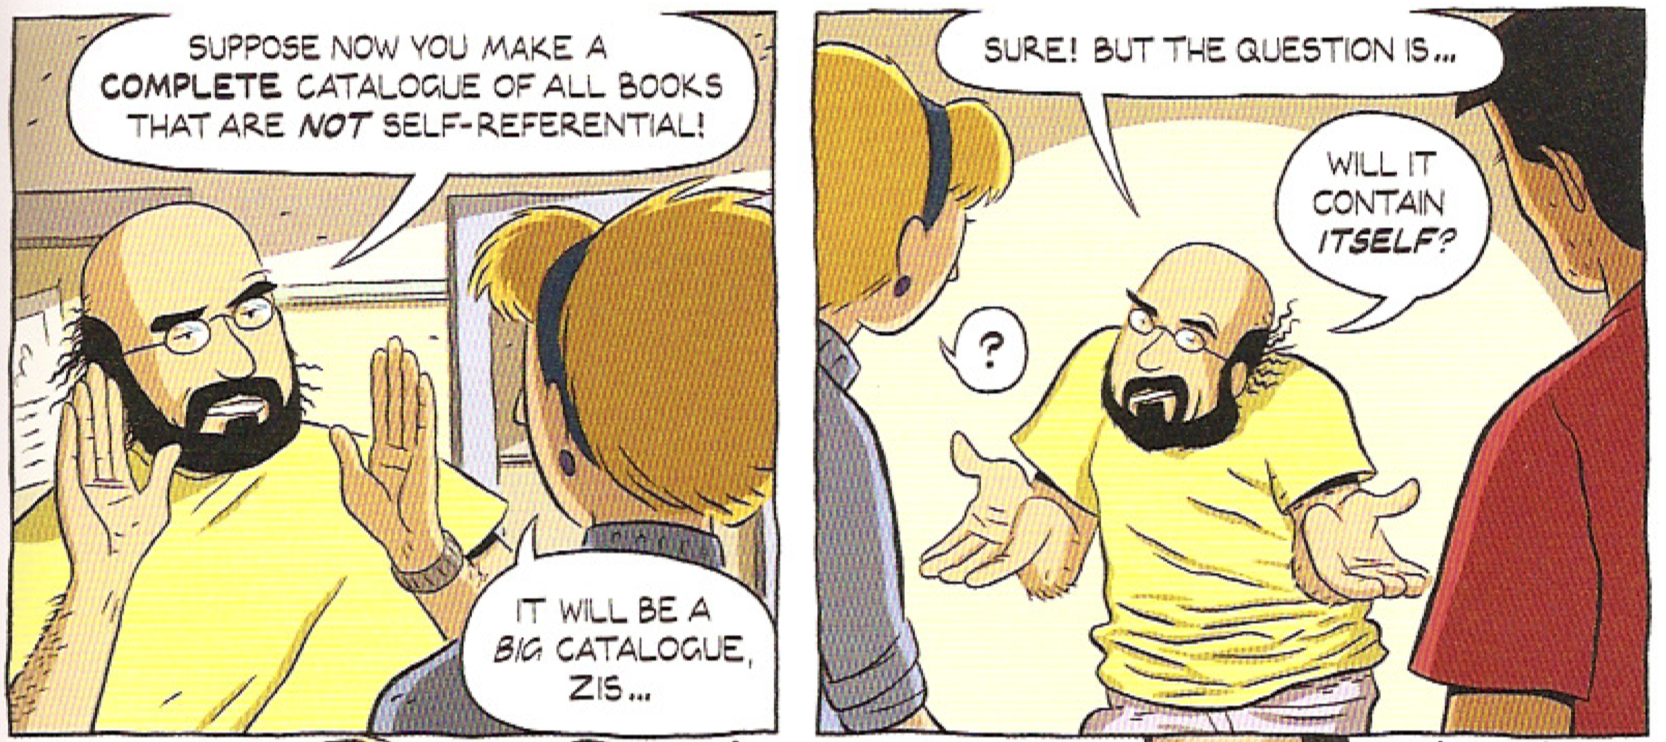
\includegraphics[width=0.75\linewidth]{logicomix.png}
    \caption{Higlighting in writing by boldface and italics in comics. Example: \textit{. An epic search for truth} \cite{logicomix}} }
    \label{fig:comics}
\end{figure}


This must suffice to illustrate the extremely important role of prosody in spoken language. But what are the acoustic features in the speech signal that are exploited to indicate what we call "prosody"? The following dimensions are commonly distinguished:  

\begin{itemize}
\item Pitch, the fundamental frequency (F0) of the vocal cord, audible over vowels and voiced consonants, like nasals. Measured in cycles per second (hertz), absolute values are speaker-dependent and therefore less important than relative values, such as high and low pitch, or pitch contours such as rising, falling, rise--fall, and fall--rise patterns.
\item Duration, the length of items, in particular syllables, measured in milliseconds. Again, relative values (like having shorter or longer duration than adjacent syllables) are more important than absolute values. 
\item Amplitude, the intensity or sound pressure levels, measured in decibels.  Again, relative values are more relevant than absolute values. 
\item Timbre, or phonatory quality, which shows up in different distributions of energy in the frequency rank, and which we will exclude from discussion here. 
\item Pauses, often related to breathing, in particular between constituents.
\end{itemize} 

There appears to be a fundamental distinction between segments and prosody: As we have seen with \ref{fig:vowelvariation}, the analog variability in the production of segments is reduced to distinct categorical phonemes (here, vowels like /i/, /\textipa{I}/, /u/, /æ/ etc. With prosody, it appears that not only the encoding is done by analogue means, but also the things that are encoded have an analogue character. For example, the more pitch is raised or amplitude is increased, the more "excited" the speaker sounds. Also, it has been argued that rules that assign stress to the syllables in syntactic phrases do so in a way that varies stress levels indefinites \cite{ChomskyHalle}, e.g. in \textit{bláckbird húnting competítion}, the stressed syllables decrease in their stress level. However, there is also evidence that what prosodic markers stand for identifies distinct categories. In particular, a prominent theoretical framework, ToBI (for "tone and break indices") \cite{beckman2006tobi} assumes a limited number of tonal phonemes like L and H for low and high tone that can be combined, e.g. LH for rising, and combinations thereof, and a use of these tonal phonemes as either nuclear accents (marked by *) or accents that indicate boundary levels (marked by \%). There is evidence that, for example, the difference between falling assertion prosody and rising question prosody is perceived categorically \cite{liu2012categorical}, and there are tunes with distinct meanings \cite{Westera2020} There is evidence that, for example, the difference between falling assertion prosody (e.g. \textit{You're coming.}) and rising question prosody (e.g. \textit{You're coming?}) is perceived categorically \cite{liu2012categorical}.

Prosody is easily seen as less central for human language, compared with segmental features. But this seems to be a misconception, due to the importance of written language. Pitch, stress, and pauses are not systematically and conventionally expressed in writing, one possible reason being that they are not perceived as categorical like phonemes. Punctuation signs like comma, fullstop, and question marks give only vague indications about prosody, and highlighting by capitalization or boldfacing is not obligatory in orthography. Their importance for spoken human language is very evident, and features of prosody have been a major topic in linguistic research (cf. e.g. the articles in Gussenhoven & Chen 2021) \cite{gussenhoven2021oxford}. However, there is less standardization in the description of prosodic phenomena than in the description of segmental phonology.

\section{Linguistic research on spoken language} 

Linguistic research on speech has a long tradition, reaching back to the 19th century \cite{levelt2013}. Due to the technical requirements, it was done in institutes and departments dedicated to phonetics. However, due to the advent of computing technology and the development of software to analyze speech data, sophisticated analyses, often based on spectrograms, could be done in regular linguistic departments. While there were predecessors, the program Praat, developed in the early 2000's, can be seen as a watershed in this development. It rapidly gained popularity, which led to the constant improvement of the program in the early years. One consequence of this was that the focus of linguistic research switched from written language (which became a topic of its own) to spoken language. 

In many cases, the main interest of researchers was not on the mechanisms of spoken language directly. Rather, the languages, language uses, and phenomena the researchers were interested could be found in the spoken modality. This included acquisition of the native language by children, acquisition of a second language, the change of language use in aging, the phenomena, like turn taking, in conversation, the use of prosodic features like stress and de-accentuation to express information structure, and the investigation of small languages and dialects that typically did not even have a written variety. For these researchers, the available tools for the acoustic investigation of spoken language can be very useful, but their application is also daunting, as they often were not trained to use them properly, and laborious, as they require minute measurements of duration, F0 changes, amplitude, and other acoustic properties, often on many entities like phonemes, syllables, words, or phrases. This could be overcome by collaboration with experts, which is often done in experimental research. But often, the phonetic tools are not used at all, or only in some limited way. (#Source?) 

The advent of automated acoustic analysis using AI techniques is another watershed moment. It has the potential for rapid analysis of relevant acoustic features of spoken language. It starts with the assistance with the transcription of speech data, often considered a time-intensive task, requiring a full hour of work for a minute of spoken data. With speech-to-text systems, this task can be simplified tremendously. However, designs that were developed for applications like dictation or subtitle creation may not be precise enough to capture the subtleties that are  the focus of researchers. For example, a researcher interested in spontaneous mispronunciation, which are an important window into speech processing, would not be happy with an output that "corrects" the data with the help of expectations triggered by the local context of the mispronounced word or syntactic constituent. Also, these devices do not give information about the precise timing of speech phenomena, like of the individual phonemes, about lengthening and shortening processes, about loudness and pitch changes. 

Hence, there is a need to make these breakthrough technologies available to researchers that work on language in their spoken variety. In the next subsection, we will turn to the results of a recent research project that shows the potential of these technologies. 


\section{Tools for investigating spoken language} 

After a very cursory overview of the structure of spoken language in segmental and supra-segmental units, we will now turn to the ways how linguistics engage with spoken languages and then will have a look at two essentials tools that are used all over the world and over several disciplines in the research of individual languages. There are alternatives, but these programs have become de facto standards for what they do. We will not mention additional auxiliary programs, such as Audacity [cite] for purposes like cutting, cleaning, and amplifying recordings. 


\subsection{Praat}

Praat is a free, open-source software for speech analysis and synthesis. Developed and maintained by Paul Boersma and David Weenink at the University of Amsterdam around 2000 \cite{boersma2001praat}, it has become a widely used standard tool for speech analysis and synthesis in phonetics, conversation analysis, sociolinguistics, dialectology and field work on endangered languages. Praat is a stable and mature workbench for the analysis, manipulation and synthesis of speech. It provides users access to waveforms and spectrograms and allows for the extraction, graphical rendering, and measuring of pitch (F0), amplitude, formants, duration, and intensity. Sound files can be annotated on multiple tiers and in a structured way. \ref{fig:praatscreen} is an example of a Praat screen with amplitude, spectrum, pitch, and various annotation tiers. Data can be exported in various ways for further analysis by statistical programs. Users can access and manipulate sounds with a GUI scripting language. Over the years, many useful scripts and routines have been developed \cite{Styler2022}. Praat has been used as a tool for the transcription of spoken languages, and it offers tools for the precise determination of landmarks and boundaries for vowels and consonants, e.g.\ identifying vowel onset and offset boundaries or measuring voice onset time in stop consonants. One slight disadvantage of Praat is that it is maintained in a somewhat irregular way and does not have strong institutional support. 


\begin{figure}
    \centering
    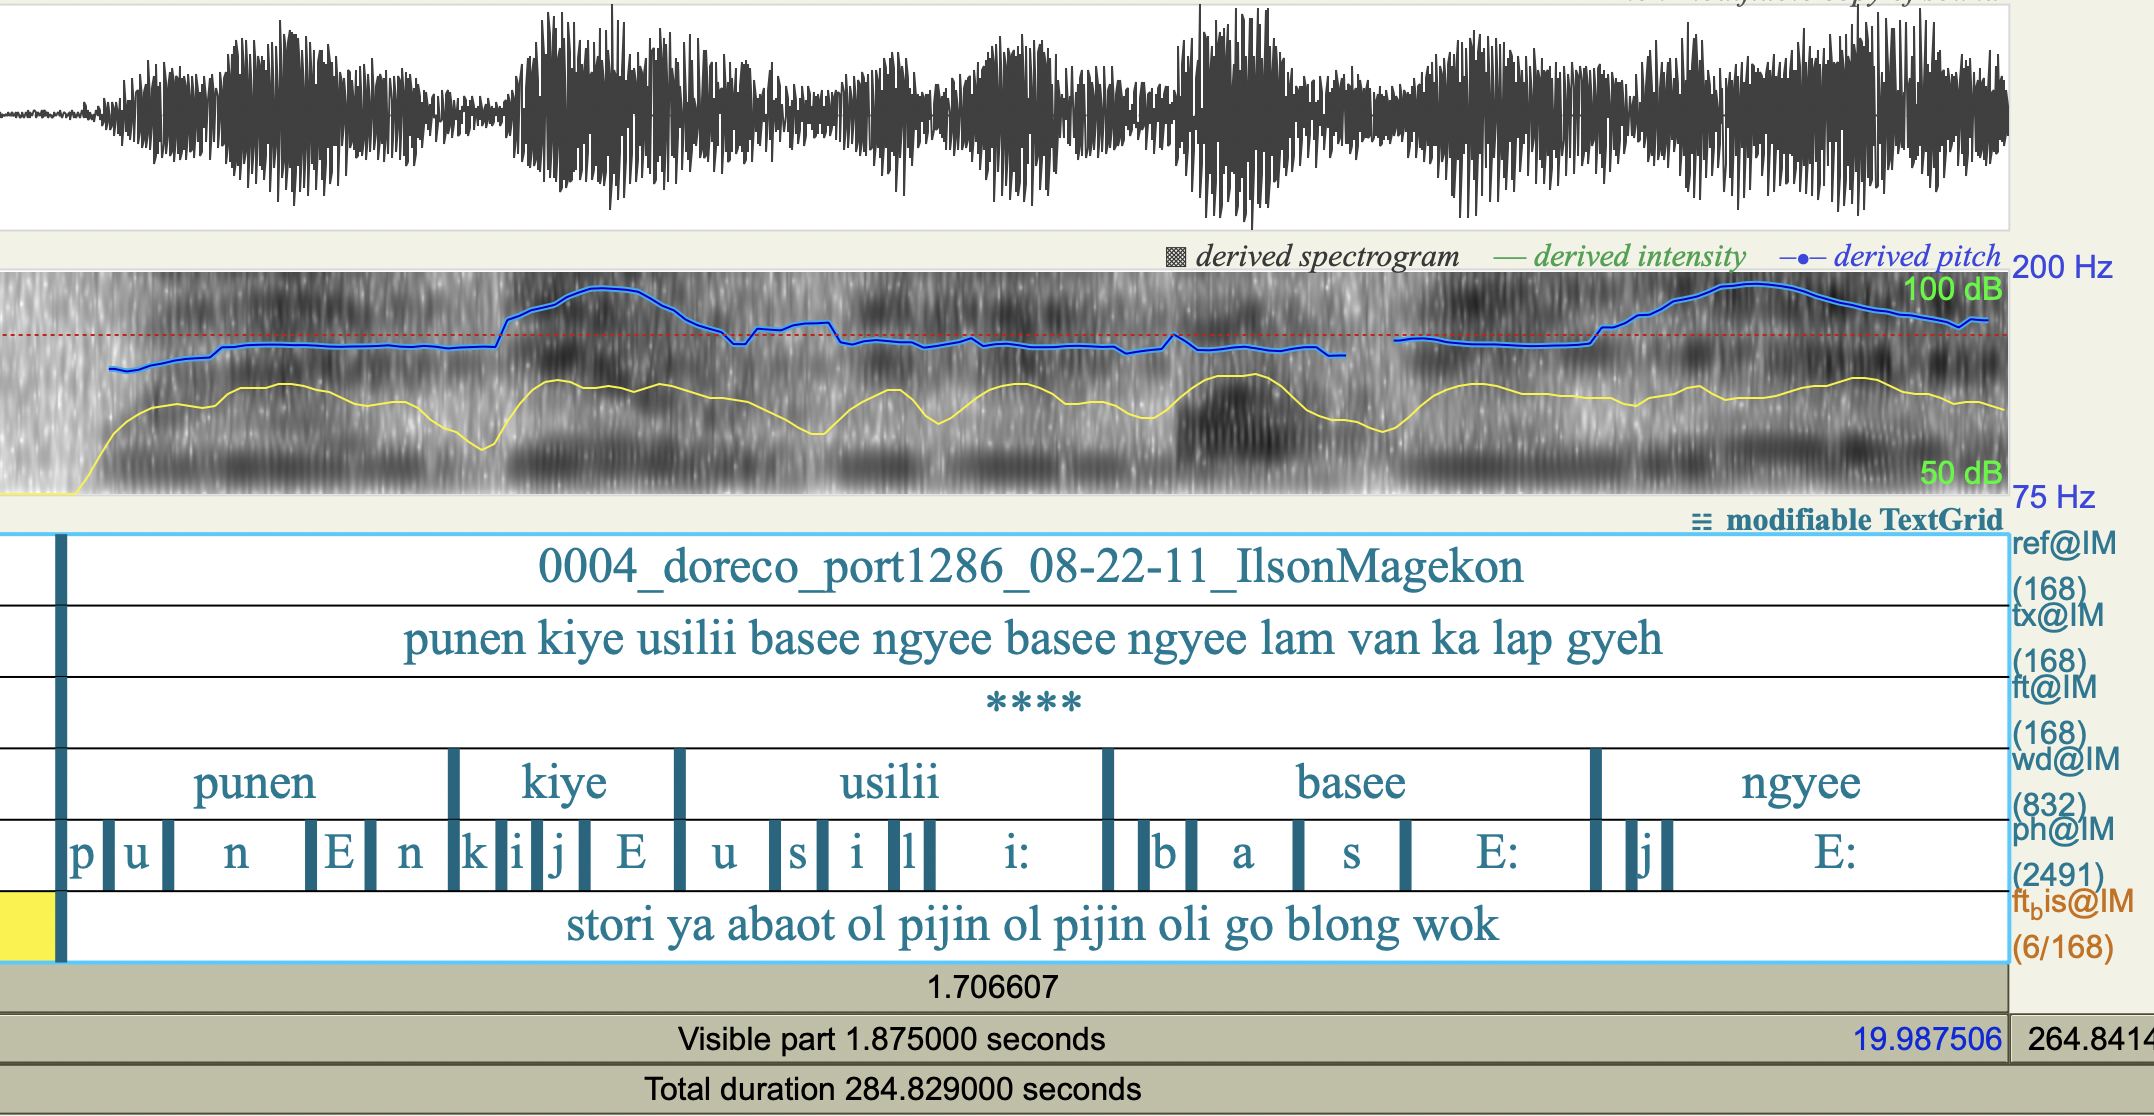
\includegraphics[width=0.95\linewidth]{praatscreen.png}
    \caption{Example of a Praat work screen, from a recording of the language Daakie (Oceanic, Vanuatu), derived from the DoReCo corpus \cite{paschen2020doreco}. From top to bottom: Amplitude, spectrogram with intensity (yellow) and F0 (blue), sentence number and recording identifier, transcription, time-aligned words, time-aligned segments and translation, here to the English-based creole language Bislama.}
    \label{fig:praatscreen}
\end{figure}

One important extension of Praat is Parselmouth, a Python library that provides access to the speech-analysis functions of Praat \cite{jadoul2018parselmouth}. Whereas Praat is normally used through its graphical interface or Praat scripting language. Parselmouth allows to perform similar functions in Python, like extract pitch/F0, intensity, formants, and duration, It can directly accesses Praat’s C/C++ code, so the algorithms and outputs are intended to match Praat itself. Parselmouth is particularly helpful in executing complex workflows in experimental research, like measuring F0, pitch range, intensity, or formats in many .wav files that contain experimental items, and saving the results in a .csv file. Thus, it integrates Praat's well-established phonetic algorithms within the broader ecosystem of Python. 

\subsection{ELAN}

Similar to Praat, ELAN was released in 2000; it was developed and is maintained by the Max-Planck Institute for Psycholinguistics in Nijmegen \cite{sloetjes2008annotation}. The focus is not on the analysis of speech but on the annotation of audio-visual events, in particular communication events. Hence, ELAN allows the work with video files, including multiple video files, that are important for the investigation of gestures, turn-taking, non-verbal communication as in sign languages, and the interaction of people with their environment. With ELAN, researchers can create a virtually unlimited number of tiers that are can be hierarchically organized. This allows for the annotation of different features of communicative events, and for different speakers. ELAN produces XML files of the type .eaf  and allows for export into more than twenty other formats.  It is highly developed for the extraction of annotation files to other programs, such as spreadsheets, statistics software, language analysis tools, and of course also Praat. It is optimized for the purposes of linguistic field work (in fact, it was used for all research projects of the DOBES project of the Volkswagen Foundation (see \url{https://dobes.mpi.nl/}) and is used in the Endangered Languages Documentation Programme ELDP (see \url{https://www.eldp.net/})). ELAN is used in a wide array of disciplines beyond linguistics, for example in psychology, education, behavioral studies, and animal communication. With the strong and continuing support of the Max Planck Society, it is continuously developed and improved with frequent updates. 

The main purpose of ELAN is to simplify and streamline the annotation of audio-visual files. There are different input formats, and tools like identifying segments for repeated listening and slowing down and speeding up recordings. It also allows for the rapid manual partition of recordings into segments that can be analyzed more deeply in subsequent steps, which is particularly important for long audiovisual files that record speech in natural environment. For each tier, separate sets of terms can be created and keyboard shortcuts can be defined, which helps to reduce the error rate in annotation. As for information about the acoustic dimension, it provides information on the amplitude and the spectrogram of the speech information. For linguistic annotation, ELAN is optimized for sentences or prosodic phrases but not for smaller parts like individual words or morphemes.  

A typical Elan screen is illustrated in Figure \ref{fig:ELANScreen}.
\begin{figure}
    \centering
    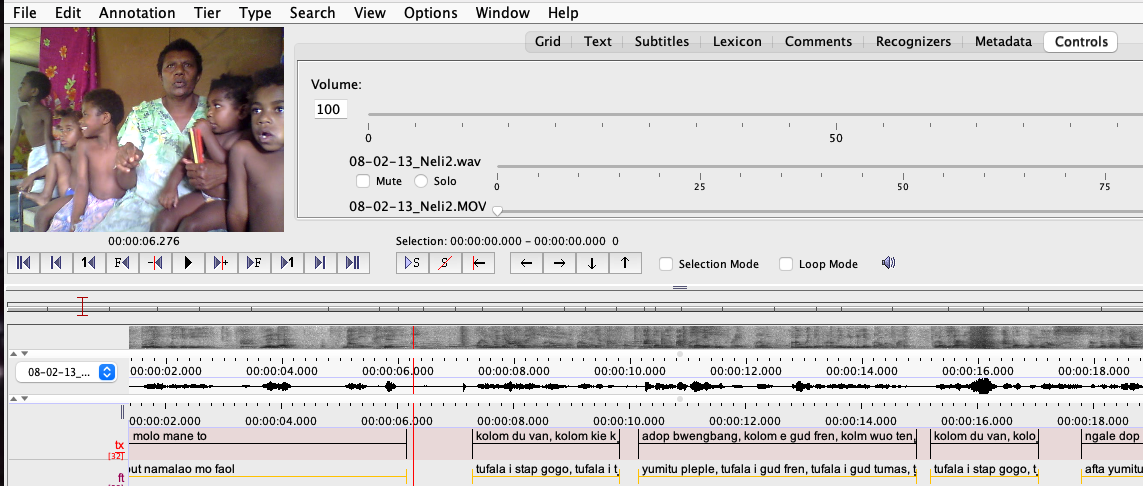
\includegraphics[width=1\linewidth]{DaakieELAN3.png}
    \caption{Cutout from an ELAN screen, with video and audio represented by a spectrum and an amplitude. Annotation tiers are original language (Daakie) and translation into the national language, Bislama}
    \label{fig:ELANScreen}
\end{figure}


\subsection{Room for improvement}

ELAN does not currently provide tools that assist researchers in the transcription of spoken language beyond showing the amplitude and a rather limited spectrograml. In particular, there is no information about pitch movement (except what is inherent in the small spectrogram), and there is no information about possible phonological segments of the language. Users interested in such more fine-grained analyses are supposed to turn to specialized tools, like Praat. While there is an export function that turns ELAN annotation files to Praat annotation files, a rapid switch from one particular point in an ELAN transcription to Praat and back again is not possible.

The current project SpeechPrint has the goal to improve this situation and provide annotators with helpful information about the segmental structure and the prosodic structure of the sound files. For this, it will make use of the techniques of automated speech recognition to pre-analyze sound data with respect to prosody and phonemes. This should results in at least two tiers, one for time-aligned phonemes, and one for pitch movement; additional tiers for syllable structures or pauses could be integrated as well. The annotations in the additional tiers don't have to be accepted at face value by the researcher but can  either serve as a source of helpful information, or can be corrected and then be used for further analysis. 

It should be stressed explicitly that a careful expert analysis with tools like Praat would provide better and more reliable results than automated techniques are able to deliver. However, the motivation of this thesis is that such techniques are useful as a support for human annotators. One could argue that human annotators could make use of existing tools, like Whisper (see below) anyway. However, linguistic field research is often done by researchers that are not trained in using such tools. For example, the Endangered Languages Documentation Project (ELDP) regularly recruits native speakers, or speakers of related languages, as researchers. While these speakers have a genuine insight in their languages, they often lack the training of using sophisticated tools. In such usage scenarios, SpeechPrint can provide some help in the crucial, and often tedious, early step of annotation.   

In order to motivate the feasibility of this goal, we will turn to a short review of automated speech recognition and the promising tools that became available, and which should be relevant for the task at hand. 

\chapter{Automated speech recognition and speech analysis tools}
\label{ASR}

In this section we will turn from the scientific investigation of spoken language and the two major research tools that are currently used for this purpose to the engineering side of recent developments. We will first contemplate on the astonishing rise of the field of automated speech recognition, and then discuss in some detail current software instruments that were developed to aid this purpose. This is meant as a survey with the intention to select the tools that could be used to achieve the goal to assist scientific research in individidual spoken languages. 

\section{Automated speech recognition}

Today (in 2026), we are surrounded by automated speech recognition technology (ASR). We expect that we can ask clients like Alexa to play a piece of music, we can communicate with an automated call center of a company, we can create subtitles of random Youtube videos, and we can converse with a person whose language we don't speak. We may no longer find this remarkable, but it took decades of intense research to reach this state. In fact, the importance of automatically transferring speech to a symbolic representation of language was identified right with the advent of digital computers. In 1952, Bell Labs built a recognizer that identified single digits spoken by a particularly speaker from the vowel formants \cite{juang2005}. By the 1980's there were the first automated type writing machines available that were trained to individual speakers. In the early 2000's, ASR began to be able to handle large vocabularies in multiple languages and independent of particular speakers, and it is increasingly used to identify speakers and their current emotional states. 

Several technological and conceptual breakthroughs were made \cite{juang2005}. One important shift around 1980 was from pattern recognition templates to Hidden Markov Models, with statistically motivated expectations for following units on the basis of preceding units. The stochastic nature of HMMs was able to cope with the high variability of spoken language between speakers and between speakers. HMMs were combined with finite state networks that allowed the identification of words and phrases. There was one problem: HMMs connect static frames, but these frames lack the uniformity of symbolic representations due to the high variability of speech data. This was solved with Gaussian mixture models that determine how well each state of the HMMs fits a frame or a short window of frames. The next breakthrough came in the early 2000's with deep neural networks. The technology of neural networks, themselves going back to the 1950's, had already been applied around 1990, but the emerging technology of deep neural networks with many hidden layers could achieve much better results \cite{hinton2012}. This allowed extensive pre-training of networks with a wide variety of inputs, essentially the same technique as with picture recognition. Newer developments feature a more general transform of acoustic features into chunks of words and phrases that avoids the phoneme level \cite{chan2015},  and the combination of convolution neural networks and transformers to model both local and global dependencies \cite{gulati2020}. Notice that these latter developments occurred within large companies like Microsoft, Google, and Amazon.

The massive technological development driven by the enormous potential economic benefit of speech recognition has led to a number of tools that are crucial for our own task, the automatic recognition of segmental and prosodic features across speakers and languages. We will turn to such tools in the following section.

\section{Speech recognizers, phoneme aligners, and prosody recognizers}

We organize this section in first looking at speech recognizers that have the goal of transferring spoken languages into orthographically represented language, typically in the standard orthography of the language. We then turn to tools that also identify the timing of the words and the individual phonemes. Finally, we will discuss tools that determine, in addition to the segmental features, prosodic features like pitch and amplitude. 

\subsection{Speech recognizer: wav2vec, HuBERT, Whisper}

We start with wav2vec 2.0 \cite{baevski2020}, a framework for self-supervised leaning of speech that trains on labeled (transcribed) data and has the goal of mapping continuous sound waves to vectors in a symbolic space.  This goal is achieved with training on a limited amount of labeled data that should be sufficient to reliably associate additional speech data with recognized words. The focus is explicitly on low-resource languages for which the training data would be limited, but the model is tested with the large dataset for English provided by the Librispeech corpus. Using the technology mentioned at the end of section, the combination of a multi-layer convolutional neural network and a transformer network for contextualized representations, the authors report that even with only 10 minutes of data, a good accuracy in phoneme recognition can be achieved.

HuBERT has the same goals as wav2vec; it enriches the speech recognition technology BERT with hidden units \cite{hsu2021hubert}.  Its underlying idea is this: Before categorical labels are available, pieces of speech are clustered into rough acoustic categories; then parts of the input are masked, and a BERT-like model is used to predict the hidden cluster labels. The important insight was that the cluster labels do not need to be perfect; they just need to be consistent enough to give the model structure. HuBERT then became useful as a strong pretrained speech encoder that could be fine-tuned for ASR and other speech tasks. 

Whisper \cite{radford2023whisper} took a different route. Instead of mainly relying on unlabeled audio plus fine-tuning, it used weak supervision, based on a large source of audio from the internet paired with imperfect transcripts, captions, translations, or other text labels. The scale and diversity of the training data were the breakthrough. The original paper emphasizes that the model generalized well to benchmarks in a zero-shot setting, often without dataset-specific fine-tuning. Architecturally, Whisper operates as a sequence-to-sequence transformer, mapping audio spectrogram features to text tokens. The process begins by resampling raw audio to 16,000 Hz and converting it into a log-Mel spectrogram with 80 channels (128 for the large-v3 model), which is then processed in fixed 30-second chunks. The encoder utilizes two 1D convolutional layers to downsample the temporal dimension before passing feature vectors to the decoder, which autoregressively predicts text tokens conditional on both the encoded audio and previously generated tokens. 

Whisper natively supports 99 languages, though its performance varies significantly based on the volume of training data; for instance, 65\% of its 680,000-hour pre-training corpus was English. This leads to high robustness for high-resource languages but creates a performance gap for low-resource, which often require fine-tuning to reach usable accuracy levels. Because the model’s byte-pair encoding (BPE) tokenizer is fixed during pre-training, adding a truly "new" language for which no token exists (e.g., specific endangered dialects) is technically challenging. Researchers can bypass this by "forcing" the model to use an existing language code as a proxy. While Whisper excels at orthographic transcription and timestamp prediction for subtitles, it does not natively produce phonetic output in the International Phonetic Alphabet (IPA). For the purposes of precise phonetic and prosodic research, Whisper must be integrated into a broader pipeline. 

The tool WhisperX \cite{bain2023whisperx} is an extension built around Whisper to overcome certain limitations. It provides more accurate timing, especially word-level timestamps, and can also provide speaker labels for recordings with multiple speakers. Based on automatic speech recognition by Whisper, it includes a voice activity detection to identify when speech is present, splitting the audio into better chunks before transcription. This is important for recordings of conversation "in the wild" (as opposed to in an experiment performed in a lab, as they often contain background noises. Cut & merge preprocessing into roughly 30-second chunks makes longer audio easier to process. Forced phoneme alignment (see the next paragraph) aligns the transcript back to the audio, producing more accurate world-level time stamps. Speaker diarization: optionally assigns speaker labels to different parts of the transcript. 

% more about languages, kind of output, IPA?

\subsection{Phoneme aligners: Montreal Forced Aligner (MFA)} 

The task of speech recognizers is to create, from spoken input, a written representation, typically using the standard orthography of a language or a narrower transcription, as in IPA. However, this does not provide information about the timing and realization of the phonemes corresponding to these graphemes in the speech signal. Such information about when phonemes and words are realized may be necessary to answer many research questions. For example, we might be interested in the distribution of pauses, the formation of prosodic phrases, the distinction between short and long syllables in languages that make this distinction, or slowing and speeding up related to the beginning or end of prosodic units. This is the task of phoneme aligners: they generally assume a transcription using an orthographic representation and provide information about the temporal alignment of these representations in the audio signal. This information can then be represented as annotation tiers in phonetic analysis programs such as Praat.

Several programs can perform this task. For example, Whisper includes a time stamp for utterances (typically an utterance surrounded by pauses, which is important, for example, for the creation of subtitles to video). To overcome the weaknesses of this component, \cite{bain2023whisperx} has developed a tool, WhisperX, that has much improved timing.program extends timing to individual words and also to phonemes. 

The most widely used aligner is MFA, the Montreal Forced Aligner, developed at McGill University \cite{mcauliffe2017mfa}. Additional documentation and downloads are available on the official website: \url{https://montreal-forced-aligner.readthedocs.io/en/latest/}. MFA is trained on a limited amount of data in several steps, first by attempting individual phoneme recognition, followed by trigram recognition, where a phoneme is identified in the context of surrounding phonemes, according to the phonological rules of a language. In the training phase, MFA performs 40 iterations in this learning phase. The MFA comes pre-trained for several languages.  The alignment was tested with the large LibriSpeech corpus for English and is reported to have fared well. As of 2026, MFA has been trained for fifty languages, with several models for some of the bigger languages. For languages not on the list it is recommended to use a phonologically similar language as a bootstrap and then train MFA on that language. The resulting time stamps are more accurate than the ones achieved by WhisperX, according to https://github.com/m-bain/whisperX/issues/1247. 

\begin{figure}[htbp]
    \centering
    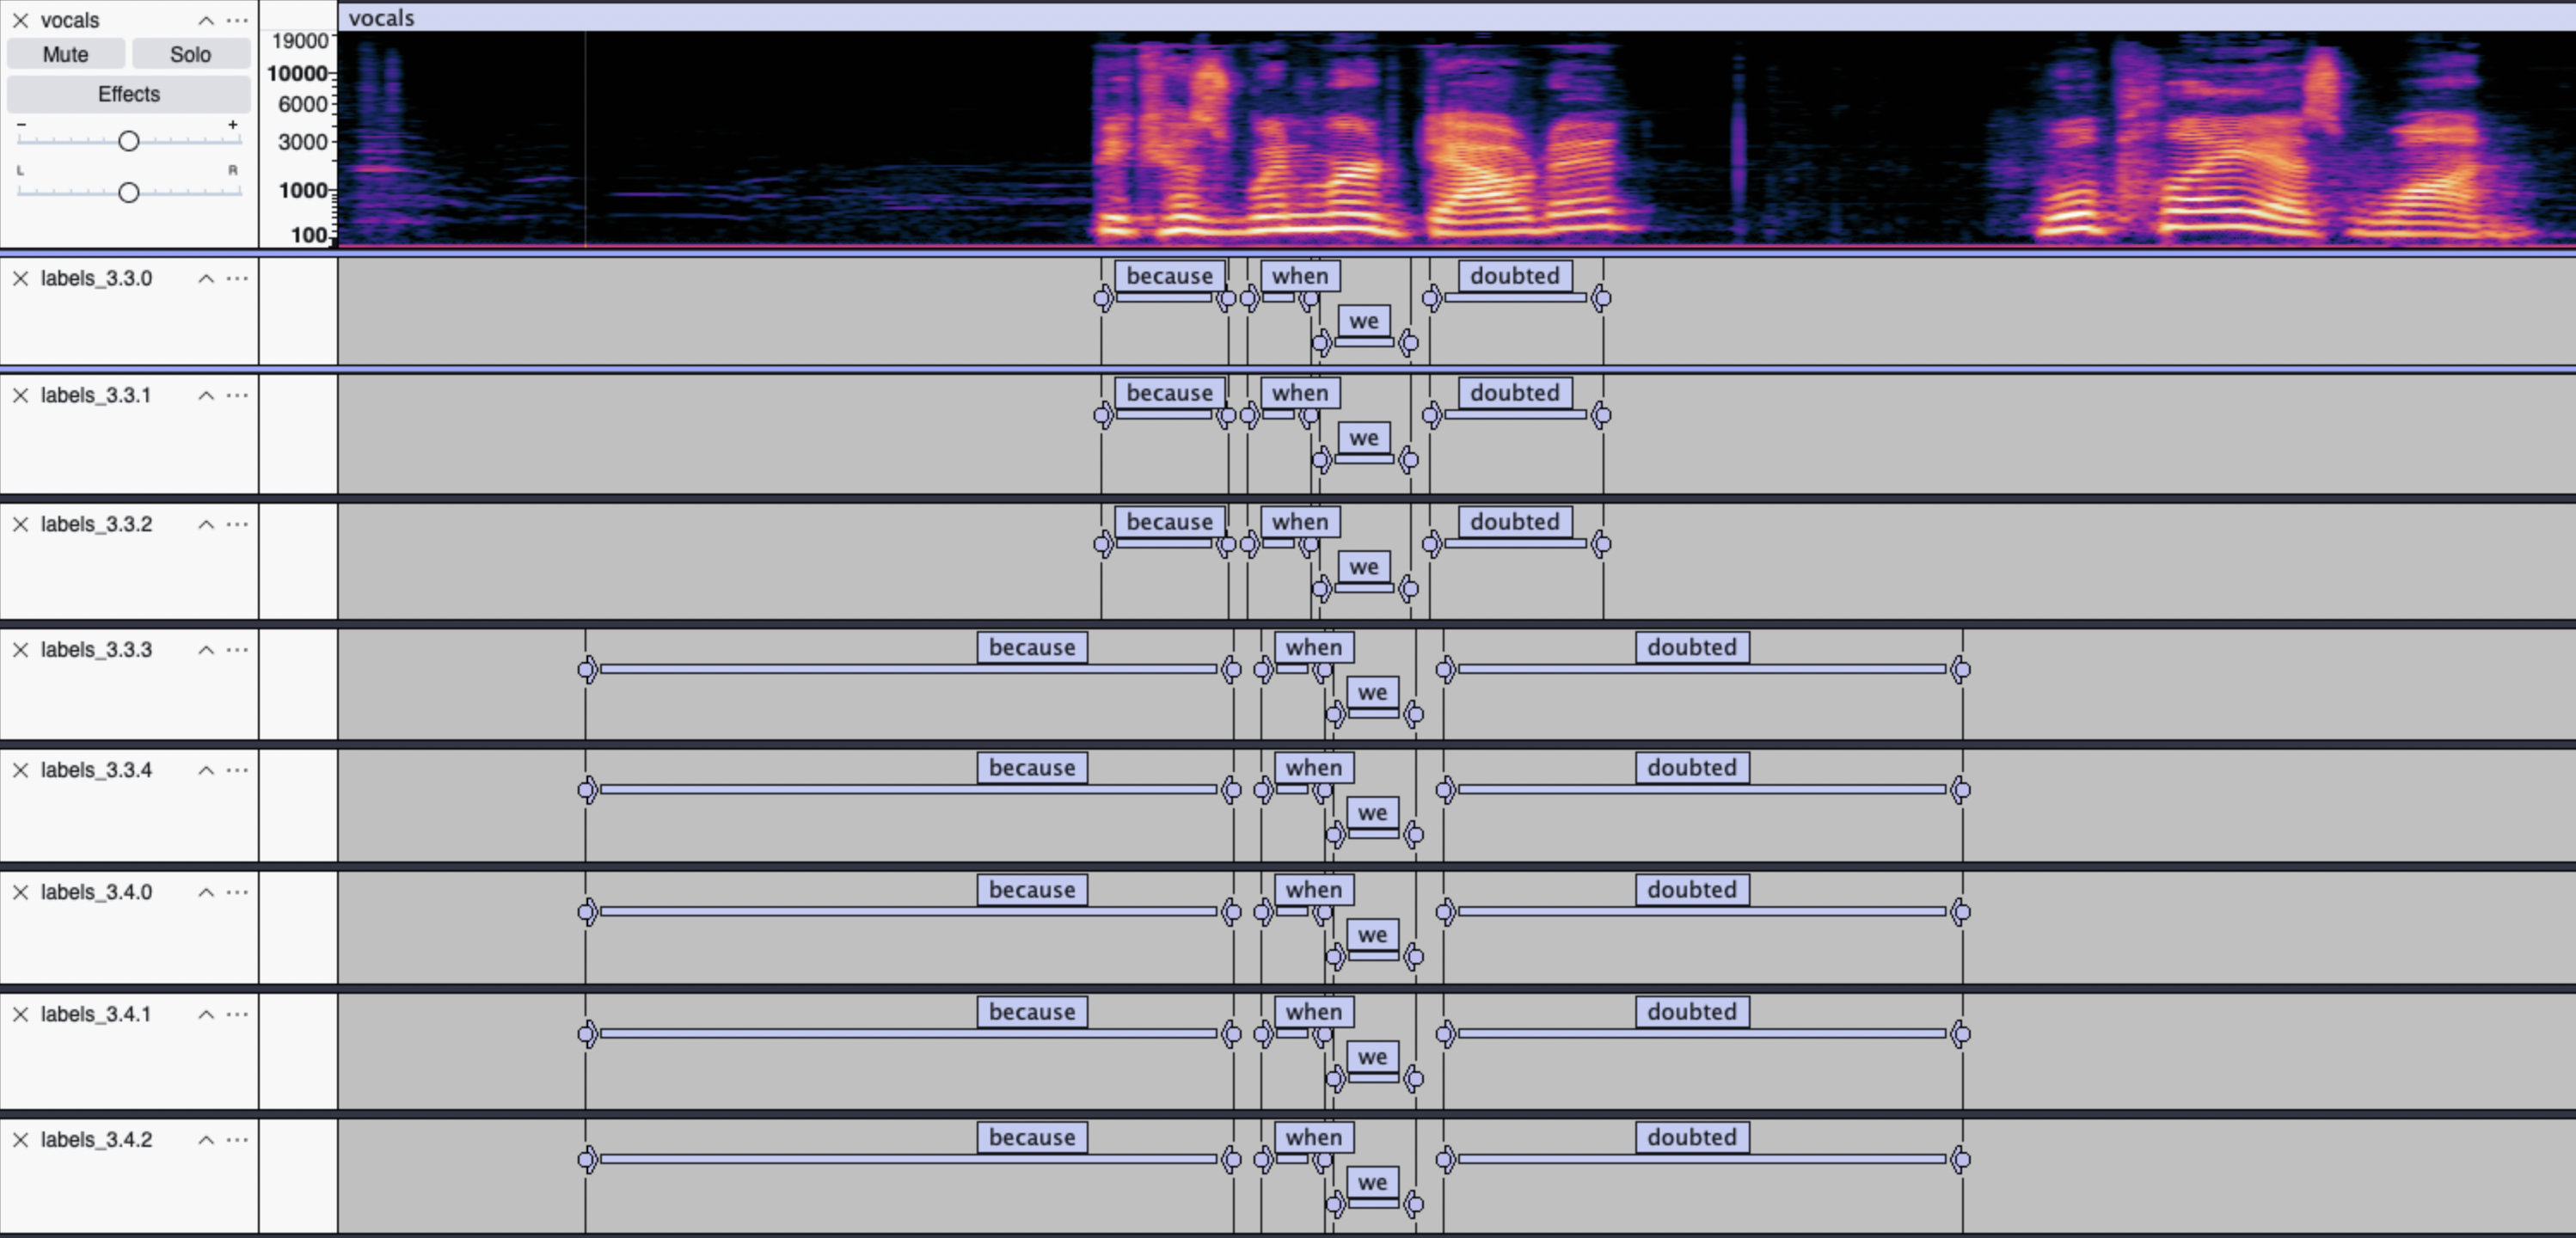
\includegraphics[width=\textwidth]{introduction/whisperx_regression_audacity.png}
    \caption{Comparative analysis in Audacity showing word-level timestamp drift in WhisperX versions 3.3.0 through 3.4.2. Note the lack of tight alignment with the audio signal following the version 3.3.3 regression \cite{bain2025whisperxissues1220}.}
    \label{fig:whisperx_drift}
\end{figure}

\begin{figure}[h]
    \centering
    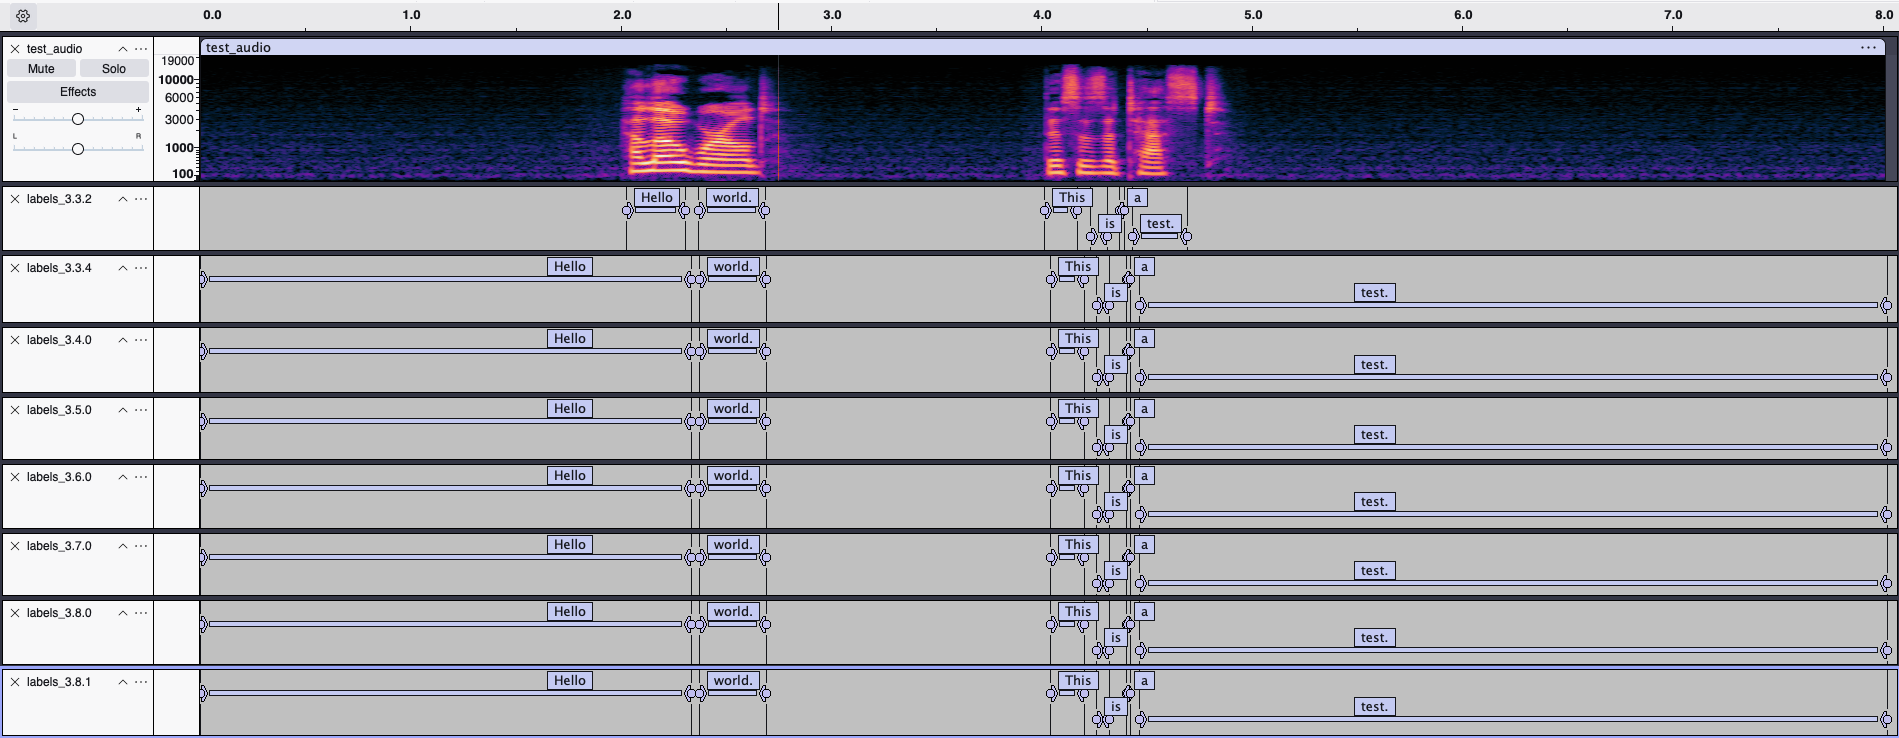
\includegraphics[width=0.92\linewidth]{introduction/whisperxfeb22.png}
    \caption{Community report documenting persistent timestamp regressions in WhisperX versions up to 3.8.1. The issue concerns premature segment triggering and alignment instability introduced after commit \texttt{69281f3}, motivating the comparative multi-aligner architecture adopted in \textit{SpeechPrint}. Source: \cite{bain2025whisperxissues1220}.}
    \label{fig:whisperx_timestamp_issue}
\end{figure}

Applying a search on the Open ASR Leaderboard \cite{srivastav2025} (current as of May 24, 2026, via Hugging Face), we identified Whisper-Large-v3 (\url{https://whisper-v3.com/} as a front runner among the open-source tools when considering the average WER, or Word Error Rate of 2.77 \% and a high number of supported languages (99). It was trained on 1 million hours of diverse, weakly labeled audio and is robust against background noise and varied accents. It shows improved performance over a wide variety of languages, showing 10\% to 20\% reduction of errors compared to Whisper large-v2.

Despite the strong alignment quality of MFA, several practical engineering limitations influenced the final design decisions of \textit{SpeechPrint}. MFA is widely regarded as ``notoriously difficult to install,'' with community discussions humorously stating that ``installing it without conda requires a priest, 10 Buddhists monks, and sacrificing 20 virgins'' \cite{bain2025whisperxissues1247}. In addition, MFA currently does not integrate naturally into lightweight \texttt{uv}-managed Python workflows used throughout this research. Furthermore, technical stability remains a concern; researchers have noted that the ``Montreal Forced Aligner... crashes with files that are longer than about 10 seconds in duration'' \cite[p. 7]{fromont2023accuracy}, necessitating the audio to be processed in ``small chunks'' \cite[p. 4]{babinski2019robin}.

The initial design designated \textbf{WhisperX} as the primary aligner to facilitate automated transcription and temporal segmentation within the framework. However, community audits and internal testing identified substantial regressions in temporal precision beginning with version 3.3.3 \cite{bain2025whisperxissues1220}. Specifically, the \textbf{integration of numerical timestamp support} was identified as the primary driver of degraded alignment accuracy; bisect results demonstrated a shift from a 0.2s baseline—the established manual threshold for distinguishing prosodic pauses in natural speech \cite{mistrorigo2018}—to a temporal error of 7.6s \cite{bain2025whisperxissues1220}. 

This loss of precision is further compounded in version 3.7.4, which exhibits instability during initial non-speech intervals. In these cases, the system frequently triggers timestamps based on \textbf{acoustic energy detection} rather than the \textbf{onset of linguistic decoding} \cite{bain2025whisperxissues1220}. This leads to premature segment initialization, a phenomenon particularly disruptive during foreign-language introductions that precede the target English speech. Because SpeechPrint requires millisecond-level accuracy to extract synchronized $F_0$ and amplitude trajectories \cite{jadoul2018parselmouth}, these regressions necessitated the development of a hybrid pipeline combining Whisper's transcription with more stable aligners like Gentle or MFA \cite{ochshorn2015gentle}, \cite{mcauliffe2017montreal}.


For this reason, \textit{SpeechPrint} ultimately adopts a hybrid pipeline combining Whisper, CrisperWhisper, and \textbf{Gentle} \cite{ochshorn2015gentle}. While WhisperX is utilized for its robust Voice Activity Detection (VAD) and batching capabilities, the framework relies on Gentle or MFA for the actual alignment. Gentle, a toolkit built on \textbf{Kaldi}, is integrated for its ``robust yet lenient'' behavior, which maintains stable long-form alignment even in the noisy field recordings typical of the \textbf{DoReCo} dataset. This design prioritizes reproducibility, maintainability, and compatibility with modern Python environments while ensuring sufficiently accurate temporal segmentation for prosodic feature extraction.

Building upon these observations, the implementation phase of \textit{SpeechPrint} focused on constructing a modular annotation environment capable of supporting multiple alignment backends within a unified workflow. The system was extended from an initially WhisperX-centered prototype into a comparative framework integrating WhisperX, Montreal Forced Aligner (MFA), Gentle, and CrisperWhisper under a shared annotation architecture.

The resulting pipeline performs automatic speech transcription using Whisper-Large-v3, followed by derivation of synchronized annotation layers including word segmentation, phoneme alignment, syllable structure, symbolic pitch trajectories, and prosodic labeling. These layers are exported as structured Praat TextGrids together with auxiliary CSV and JSON metadata for downstream inspection, correction, and evaluation.

To support comparative alignment analysis, a generalized aligner abstraction layer was introduced. Each backend was normalized into a shared representation containing lexical intervals, optional phone-level data, timing metadata, and diagnostic warning states. This restructuring enabled the pipeline to interchange alignment strategies without requiring modifications to downstream processing stages.

Particular engineering effort was devoted to the integration of Montreal Forced Aligner. Due to repeated instability in pip-based installation workflows, a dedicated Miniforge and Mamba environment was introduced to ensure reproducible installation of OpenFST, \texttt{pynini}, \texttt{kalpy}, and multilingual acoustic models. The language mapping infrastructure was additionally expanded to support multilingual corpora beyond English.

Gentle was integrated through its native HTTP server architecture rather than embedding Kaldi directly into the primary Python environment. This separation reduced dependency conflicts and simplified deployment while preserving compatibility with lightweight \texttt{uv}-managed workflows used throughout the project.

The graphical interface was extended conservatively in order to preserve the existing annotation workflow. Additional controls were introduced for aligner selection, comparative alignment analysis, and Praat export management. The system additionally gained support for generation of per-aligner TextGrids and comparison CSV outputs intended for evaluating temporal divergence between alignment models.

The resulting environment provides synchronized visualization of waveform, spectrogram, formants, intensity traces, symbolic pitch representations, phoneme segmentation, syllable structures, and aligned lexical units within Praat.

The comparative alignment subsystem was intentionally separated from the canonical analytical representation used for downstream processing. Rather than collapsing all aligner outputs into a single averaged representation, each backend was preserved as an independent lexical hypothesis within Praat. This resulted in parallel tiers such as \texttt{words\_whisperx}, \texttt{words\_gentle}, \texttt{words\_mfa}, and \texttt{words\_crisperwhisper}, allowing direct inspection of temporal disagreement between alignment systems.

This distinction became particularly important during evaluation of WhisperX regressions introduced after version 3.3.3, where word onsets occasionally drifted several hundred milliseconds from the acoustic signal. By preserving multiple alignments simultaneously, the system could expose segmentation instability visually rather than concealing it behind a single forced representation. Comparison CSV files containing timestamp deviations and mean absolute deviation (MAD) measurements were additionally generated to support quantitative auditing of aligner disagreement.

However, higher-level linguistic tiers such as phonemes, syllables, symbolic pitch trajectories, and prosodic labels were not derived from averaged alignments. While lexical boundaries can be compared numerically across systems, phoneme segmentation represents a categorical symbolic decision rather than a continuous measurement. Averaging phonetic boundaries across multiple backends would therefore produce artificial intervals not predicted by any individual model.

For this reason, \textit{SpeechPrint} adopts a canonical alignment strategy for downstream analysis. A single primary aligner is selected for derivation of phoneme intervals, syllable structure, \(F_0\) extraction, and symbolic prosodic annotation. MFA is preferred whenever available due to its phone-level acoustic modeling, while Gentle or WhisperX are used as fallback solutions depending on runtime availability and language support.

This separation between comparative and canonical layers simplified the engineering architecture considerably. The comparative tiers function as an evaluative and diagnostic layer, whereas the canonical representation provides a stable substrate for subsequent acoustic analysis, corpus evaluation, and generative transformations.

These extensions established the technical foundation required for subsequent evaluation experiments on multilingual and long-form speech corpora.

\subsection{Choice of Languages and Datasets}

The selection of high-resource European languages---specifically English, German, Italian, Spanish, French, and Czech---serves to validate the framework across diverse phonetic architectures. Czech is particularly illustrative for this research, as its vowel nuclei can be formed by liquids and nasals, as in \textit{vlk} (wolf) and \textit{prst} (finger) \cite{paschen2020doreco}. This provides a rigorous test for the system’s ability to automate vowel identification in phonetically complex environments.

By utilizing a dataset that pairs ``spoken'' and ``sung'' versions of these languages, such as Lorca’s poetry or Poe’s \textit{The Bells}, the system analyzes how melodic modulation affects transcription accuracy. This dataset supports the ultimate goal of achieving a state where ``95\% it works,'' treating speech as ``Dynamic Vector Graphics'' to preserve the rich prosodic and phonetic architecture of human performance.

To ensure scientific rigor beyond high-resource languages, the pipeline is benchmarked against the DoReCo (Language Documentation Reference Corpus). DoReCo is a hand-annotated, time-aligned cross-linguistic reference corpus containing 53 small, under-resourced languages \cite{paschen2020doreco}. These files are considered the academic ``gold standard'' because they were hand-checked by experts over several years. This comparison allows for a terminal-based ``Stress Test'' where any temporal offset greater than 20\,ms is flagged as a failure, providing empirical evidence that AI-driven alignment can approach the precision of human experts within an engineering-focused framework.

\subsection{Technical Realization and Tool Trade-offs}

The technical implementation of the SpeechPrint utilizes a hybrid pipeline combining Whisper, CrisperWhisper (Faster Whisper), Gentle, and MFA. While OpenAI Whisper provides a robust multilingual foundation \cite{radford2023whisper}, Gentle---a toolkit built on Kaldi---is integrated for its word-based granularity, which remains effective even in the noisy field recordings typical of linguistic documentation.

The decision to use a multi-tool approach stems from the inherent disadvantages of MFA. Although MFA is highly accurate \cite{mcauliffe2017mfa}, it is notoriously difficult to install, with community consensus humorously noting that ``installing it without conda requires a priest.'' Furthermore, MFA does not natively support the modern \texttt{uv}-managed Python environment preferred for this research. By using WhisperX \cite{bain2023whisperx} or Gentle to provide an initial timing scaffold, the framework avoids the tendency of MFA to crash with files longer than approximately 10 seconds. This ensures that the pipeline remains stable for the long-form narratives found in the DoReCo corpus and the European poetry datasets.

\subsection{Prosody recognizers: ProsodyPro}

To investigate prosodic features of language, Praat is the research tool of choice because it provides easy and reliable access to pitch height (F0 movement), duration, and amplitude (# ref above). Various tools have been developed to assist researchers in prosodic research using Praat. 

In particular, ProsodyPro \cite{xu2013prosodypro} is a Praat script/toolkit for semi-automatic prosodic analysis of speech that is used to extract pitch-related measures such as F0 contours, mean F0, pitch range, and duration, and possibly intensity over user-defined intervals, often vowels, syllables, words, or larger prosodic units that are already annotated. Its particular strengh is with batch processing to simplyfy work with experimental data. A more recent tool is Parselmouth, \cite{Jadoul2018},  \url{https://parselmouth.readthedocs.io/en/stable/}, a Python library that directly accesses the Praat code. 

In addition to established tools such as ProsodyPro and Parselmouth, the phonetic research landscape includes several specialized frameworks for large-scale data management and acoustic feature extraction. The EMU Speech Database Management System (EMU-SDMS) functions as a robust annotation and database framework specifically designed for managing large annotated speech corpora and querying phonetic or prosodic data \cite{winkelmann2017emu}. 

For broad-spectrum feature extraction, OpenSMILE remains one of the most widely used standards for ``large-scale acoustic feature extraction'' \cite{eyben2010opensmile}. It is commonly employed for extracting pitch, intensity, spectral, emotional, and voice-quality related descriptors across large multilingual datasets. When research questions require higher spectral resolution and voice-quality analysis, tools such as PraatSauce or VoiceSauce are frequently utilized to measure H1-H2, spectral tilt, formants, and F$_0$ contours \cite{shue2011voicesauce}. 

Earlier generations of automatic prosodic annotation tools, such as AuToBI \cite{rosenberg2010autobi}, focused primarily on the detection of ToBI-style pitch accents and prosodic boundaries. While influential in computational prosody research, these systems are increasingly viewed as part of an earlier methodological generation that predates modern neural-based speech pipelines and large multilingual transformer architectures.

The SpeechPrint framework prioritizes a more modern pipeline architecture centered around WhisperX, MFA, Gentle, and Parselmouth. In this design, Whisper-based systems provide rapid multilingual transcription and Voice Activity Detection (VAD), creating an initial ``timing scaffold'' for downstream processing. To obtain temporally precise phoneme and word boundaries, forced alignment systems such as MFA or Gentle are then employed to generate Praat-compatible TextGrids with near millisecond-level precision \cite{mcauliffe2017mfa}. 

The final extraction of ``etic'' acoustic features is performed using Parselmouth, a Python interface to Praat that exposes Praat’s internal phonetic analysis algorithms directly within programmable workflows \cite{jadoul2018parselmouth}. This integration is prioritized over older Praat scripting approaches such as ProsodyPro because Parselmouth integrates naturally into Python-based machine learning and data analysis environments. Through this architecture, SpeechPrint can automatically generate multidimensional feature representations containing F$_0$ (pitch), duration, intensity, spectral information, pause structure, and amplitude measurements suitable for both scientific analysis and artistic visualization.

A central design philosophy of SpeechPrint is the treatment of speech as a form of ``Dynamic Vector Graphics,'' where temporally aligned phonetic units become navigable structural objects for computational analysis, clustering, and audiovisual representation. By combining multilingual ASR systems with forced alignment and programmable acoustic analysis, the framework maintains reproducibility and fine-grained control over temporal error thresholds while remaining adaptable to under-resourced languages and long-form recordings.


\chapter{A new tool: SpeechPrint}
\label{speechprint}

\section{Motivation}

# There exist very valuable tools, often not straightforward to use for working linguistics, e.g. conversation analysts, field linguistc etc. beyond phoneticians and specialists in spoken languages
# Goal: Provide a tool that can be the basis for researchers, also useful for artful visualizations of speech; should be easy to understand; for example, easy integration into existing annotation tools like ELAN
# Essential: should combine information about segments (phonemes), syllables, pauses, and prosody, as these are essential features for further analysis of speech. 
# Measure of success: (a) Benchmark with existing analyzed recordings, (b) asking working linguistics how they experience the system, how useful it would be for them. 

\section{Phoneme identification}

# Describe the choice of tools that you are using (most probably targetting Whisper; if others, describe why you select them; describe how good these tools are with your benchmark files. 

# Settle on one particular program (or have alternatives?). Say how to set parameters for the program, e.g. for different languages and for languages that are not recognized. Show the outputs for the benchmark date that are used

\section{Rendering of Prosody}

# Identify the data that you want to get: Syllable boundaries (from vowels and adjacent consonants?) In particular: F0 and amplitude information of the vowel parts, using the input from the phoneme identification. 

# Discuss ways of rendering prosody graphically. Propose one intuitive system to use: F0 movement / _ -- backward slash for F0, Star * for stress/amplitude, perhaps | for pauses?

# Show the output of the prosodic analysis for benchmark files, have experts judge how close they are to proper analysis by humans. 

\chapter{Testing SpeechPrint}
\label{testing}

\section{Choice of languages and recordings}

# Here: motivate the choice of languages (5 European languages, 5 Non-European languages) and the choice of genre (Narratives, ideally 3 per language, by different speakers, about 1 minute per language). For these I will take DoReCo data. I will check which Whisper settings are particularly good for particular languages and write down recommendations. 

When testing a tool, we require something that can be said to represent the "objective truth". For SpeechPrint, this will consist in two parts: First, we will have to test the accuracy of the identification and the timing of phonemes. Secondly, we have to consider possibilities to adjucate how well the tool is dealing with prosody. In this section, we will turn to these tasks. 

\section{Benchmarks for phoneme identification and alignment}

As for the identification of phonemes, there are several options. Phoneme identification is crucial for speech-to-text systems that transfer spoken language to a written representation in the standard orthography of a the language, hence industrial-strenght benchmarks have been developed for this tasks. #cite. Our purpose is different, as we would like to see how SpeechPrint fares with small languages for which resources like large and diverse benchmarks do not exist. However, for this purpose there exists a tool: The DoReCo corpus. 

\subsection{Small languages: DoReCo}

DoReCo, the Language Documentation Reference Corpus \cite{paschen2020doreco}, see \url{https://doreco.info/}, is a multilingual, time-aligned corpus built from language-documentation materials, especially fieldwork-based corpora of small, under-resourced, and often endangered languages. The current DoReCo site describes version 2.0 as covering a worldwide sample of 53 languages with over 100 hours of  mostly narrative audio, phone-level time-aligned transcription, translations. For 39 languages, there is also a time-aligned morphological annotation. 

The basic idea is to make language-documentation data usable for broader comparative research. Many fieldwork archives contain rich audio and transcripts, but they often differ in file formats, annotation conventions, and time-alignment detail. The DoReCo project standardizes these materials and adds finer-grained time alignment, allowing researchers to ask cross-linguistic questions about speech timing, phonetic lengthening, morphology, information rate, pauses, and narrative structure \cite{paschen2020doreco}. The corpus is particularly valuable because the data are not artificial word lists or isolated elicited examples, but spontaneously produced traditional or personal narratives, as well as conversations and stimulus retellings. The original language experts selected particularly good recordings that were transcribed, translated, and often morphologically annotated before their inclusion in DoReCo; the DoReCo project then harmonized the structure and added time alignment of phones, words, and, where available, morphs. 

The annotation formats include ELAN, Praat, TEI, and CSV. The ELAN .eaf file serves as the master format from which the others are generated. Time alignment was carried out with the aligner WebMAUS \cite{kisler2012webmaus} and then carefully hand-corrected by a large German-French research team over the course of several years. Hence, it can be considered one of the most carefully time-aligned multilingual corpora currently available for under-resourced and endangered languages. For this reason, it provides a particularly useful benchmark for the current project. In the present work, five languages from the DoReCo corpus were selected for evaluation. However, while the DoReCo corpus is aligned at the level of phonemes, words, and morphs, it does not contain dedicated annotation tiers for prosodic phenomena such as intonation, stress, or pitch movement.

DoReCo differs substantially from classic speech corpora such as TIMIT and Buckeye. The TIMIT corpus was designed primarily for phonetic and automatic speech recognition research in American English and contains carefully recorded read sentences with highly controlled phonetic transcriptions. The Buckeye Corpus, by contrast, contains spontaneous conversational American English and is particularly valuable for the study of reduction phenomena and natural speech variation. While these corpora are highly influential and widely used benchmarks in speech technology research, they focus almost exclusively on English. DoReCo extends this type of work into a strongly multilingual and language-documentation-oriented setting, including many endangered and typologically diverse languages from different parts of the world.

\section{Benchmarks for prosody}

# ToBI
# Prosodic Minimal Pairs

While automatic speech recognition traditionally focuses on orthographic accuracy, recent linguistic and computational research has increasingly made use of ``prosodic minimal pairs'', short utterances that differ primarily in prosody rather than in their segmental structure. Such pairs are useful because they isolate how communicative intentions are expressed through pitch, stress, duration, rhythm, and emphasis while keeping the lexical material largely constant. This is particularly relevant because written text is often an impoverished representation of spoken language, lacking direct information about intonation, prominence, emotional coloring, or information structure \cite{nguyen2023expresso}.

One line of research investigates focus prosody. For example, utterances like \textit{I did it} may receive prominence on different words depending on the communicative context, changing the interpretation of the sentence. Similarly, lexical stress doublets such as \textit{object} (noun) versus \textit{object} (verb) demonstrate how shifts in stress placement correlate with grammatical categories. Recent benchmark work by Rooth and collaborators investigates such phenomena systematically using large collections of naturally occurring recordings gathered from online sources \cite{lagisetty2026ml}. 

Other recent benchmarks focus on more specific dimensions of prosody. The Prosodic ABX dataset compares contrasts such as lexical stress, pitch accent, and lexical tone across several languages, including English, Japanese, and Mandarin \cite{sun2025prosodic}. The EmphAssess benchmark investigates the preservation of emphasis by comparing sentences in which only the emphasized word changes \cite{cassini2024emphasis}. These benchmarks are intended to evaluate whether speech representations preserve prosodically relevant distinctions that are important for meaning.

An important observation emerging from this work is that prosodic interpretation is often difficult even for modern machine-learning systems. For example, contextual language models such as BERT perform relatively poorly on the prediction of contrastive focus because these distinctions often require semantic, pragmatic, or discourse-level interpretation \cite{stephenson2022bert}. In many cases, the same sentence can receive several equally plausible prosodic realizations depending on the speaker's communicative intention.

This is relevant for the current project because SpeechPrint is not intended merely as a transcription tool, but also as a way of visualizing systematic relationships in speech data. Prosodic minimal pairs provide a useful testing ground because they make it possible to investigate whether small changes in prominence, stress, or intonation produce visible and interpretable changes in representation space. In this sense, they function as controlled benchmarks for evaluating whether visualization methods preserve meaningful prosodic structure.

\subsection{Testing prosody identification}

# Prosodic benchmarks
# Using your own set of prosodic minimal pairs

\section{Results of the testing for the individual languages}

\subsection{German: GToBI}

In this section we will test SpeechPrint with a few example sentences in German that were annotated according to the ToBI. They are retrieved from the GToBI instruction site developed by the University of Cologne, \href{http://www.gtobi.uni-koeln.de/}{http://www.gtobi.uni-koeln.de/}. They are expertly annotated using the ToBI system adapted for German. These are single phrases or sentences in which a particular tone contour is illustrated, so they only provide an annotation of the nuclear accent and a boundary tone. 

\begin{figure}
    \centering
    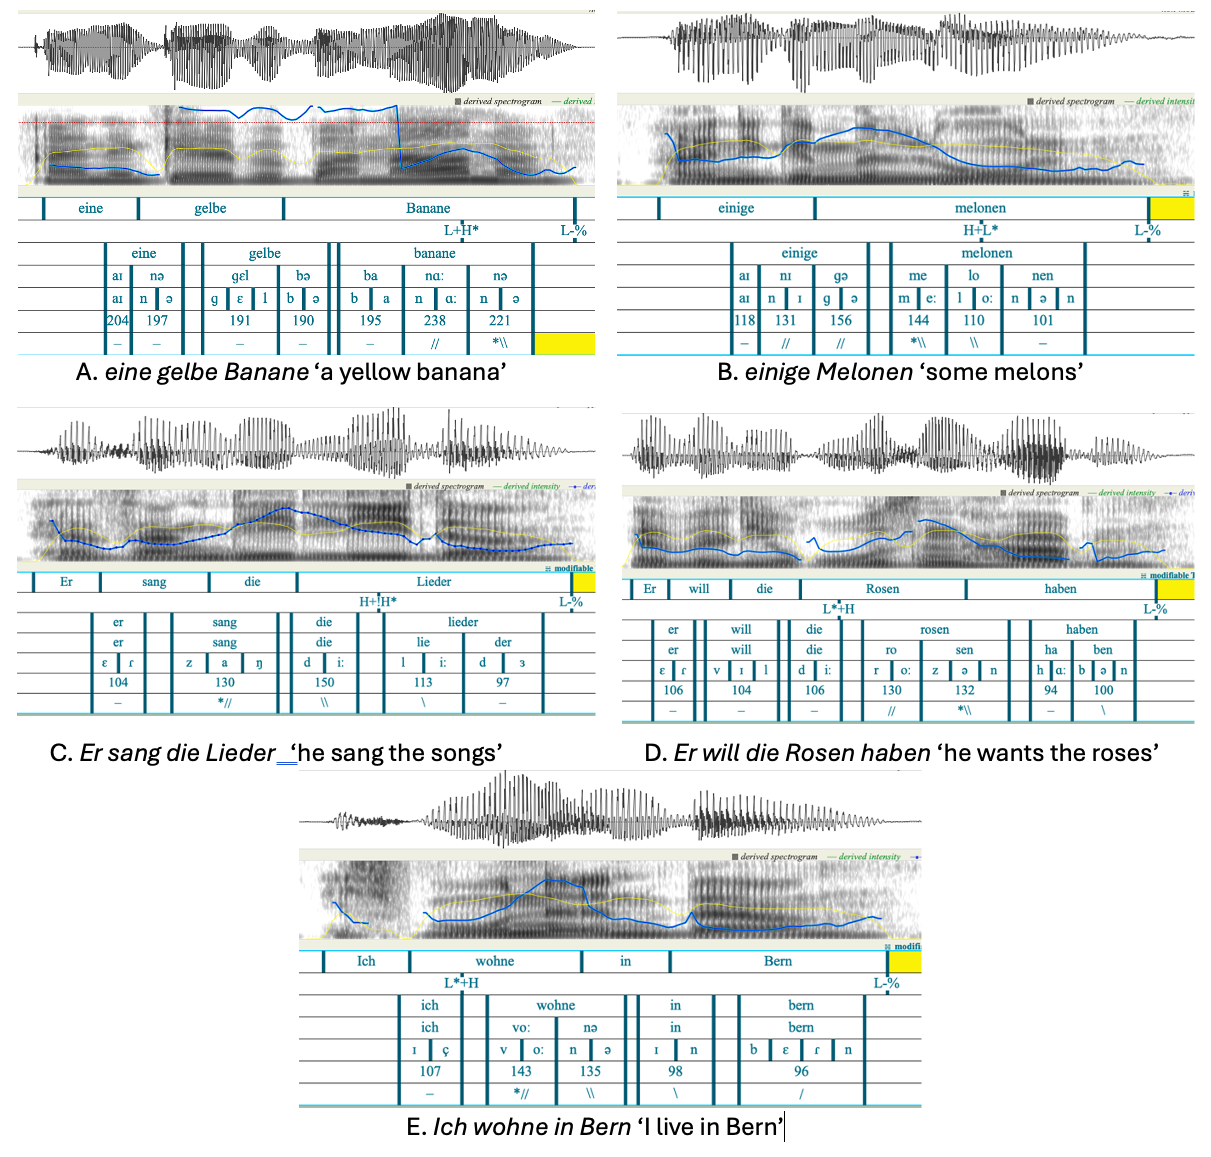
\includegraphics[width=1\linewidth]{image.png}
    \caption{Five recordings of example sentences annotated following the GToBI convention. Wavelines and spectrogram are shown, the spectrogram also contains information about pitch (blue) and amplitude (yellow). Line 1: orthographic rendering, 2: GToBI annotation, 3: individual words, 4: syllables, 5: phonemes, 6: syllable length in ms, 7: pitch and intensity representation by SpeechPrint}
    \label{fig:gtobi}
\end{figure}


The GToBI annotations (second line) were the only information provided. SpeechPrint was applied with WhisperX using the big German model (the small model gave insufficienct results). This generated orthographically correct representations, as expected. The individual words were also generated correctly; however, their timing often is off, especially at the beginning of the phrase (e.g. the onset of \textit{eine} in A is considerably delayed). This is a known problem (ref. #). The individual syllables and phonemes are well represented; however, the individual phonemes are not time-aligned. The numeric length of the syllables appear to be correct (e.g. \textit{ei-ne} as 204ms and 197ms, contradicting the visual representation by the hairlines). 

The representation of prosody is generally quite good. A has a rising-falling contour L+H* L-\% that is represented by // and \textbackslash \textbackslash. Here the identification of the main stress is off by one syllable (\textit{ba'nane}). B has a falling contour H+L* L-\%. This is also well represented, where the rise builds up in the preceding syllables // and the fall is expressed by \textbackslash \textbackslash. Again, the main accent * is not quite right, it should be on \textit{me'lone}. C is an instance of downstep H+!H* and low boundary tone L-\%. The pre-accent rising is well represented, and so is the falling. There should be an accent mark * on \textit{Lieder} as well, however. D represents a rising accent L*-H followed by a low boundary tone L-\%, which is well represented by // \textbackslash \textbackslash\; however, the accented syllable is again off, as it should be {'rosen}. E is a case in which \textit{wohne} ‘live’ is highlighted and carries a L*-H accent; this is perfectly represented by *// followed by \textbackslash \textbackslash. 

This test shows that with a high-resource language and exemplary recordings, the results provided by SpeechPrint are quite accurate. They provide a helpful tool for further analysis. The main problem, it appears, is with the temporal alignment of syllables and phonemes. 



\chapter{Use scenarios}
\label{scenarios}

\section{Scientific use scenario}

% Show how the features of phoneme and prosody identification can be bundled in one tool, show how this tool is made useful for users, perhaps give a user-friendly description of the tool. Discuss various output formats, in particular ELAN annotation files with two tiers. 

% Evaluate this with linguists that work in field work and/or conversation analysis. 

\section{Aesthetic use scenario}

Representation of speech print to visualize sound structure of aesthetic texts, in particular poems. 

\section{Further developments}

Possible use of an easy to understand prosodic annotation for text-to-speech systems. Here one would have to talk about the problem of prosody for text-to-speech, and do some research on this problem. This could be interesting if the rendering of prosody is considered intuitively easy and satisfying. 





A core contribution of the project is a richly annotated speech corpus Doreco, recorded with native speakers, covering a broad range of speaking styles, affective states, hand annotated voice maps are created to identify word, syllable and phoneme boundaries for each speaker to identify phonation regions and guide modelling of voice quality dimensions such as creakiness and breathiness. The corpus and voice profiles have been released as open-source resources for the research community.


SpeechPrint: A Tool for Extracting Phonemic and Phonetic Information, with Usage Scenarios in Science, Technology, and Art

The core of the project is the development of a tool that transforms human speech into a representation that combines symbolic information that is usable for different purposes. Existing tools like Whisper, HuBERT and Allosaurus provide for categorical (qualitative) information about the orthographic or phonemic representation that is required for Speech-to-Text systems \cite{radford2023whisper,hsu2021hubert,li2020allosaurus}.These tools can also provide quantitative information about the temporal location and duration of phonemes, though this information is often unreliable. The tool I want to develop adds several quantitative measures, in particular the pitch and amplitude of vowels and diphthongs. In this, it combines phonemic and phonetic information, which motivates the term “EmEt,” following the coinage of the “emic” and “etic” approaches by the linguist Kenneth Pike \cite{pike1967language}. I believe this information would be useful for many usage scenarios in science, technology, and art.

The EmEt tool should allow for WAV files in specified languages as input. Optionally, orthographic representations can be provided as well for usage scenarios like read speech, recited poetry or songs. The output consists of a phonemic representation aligned with a classification of the phonemes (vowels, diphthongs, different classes of consonants), time stamp information about the phonemes, and, for vowels and diphthongs, information about F0 and amplitude. From this, timestamps identifying syllables and pauses, identification of accented syllables, and classification of accent types (like falling, rising, high, low) can be derived and will optionally be part of the output files.

I constructed a first prototype after testing various existing tools. I combined several tools: WhisperX for the transcript \cite{bain2023whisperx}, a phoneme-aware forced aligner for phoneme timestamps, and additional acoustic extraction for F0, formants, and amplitude using Parselmouth \cite{jadoul2018parselmouth} (Praat for Python). Espeak \cite{espeakng2024} was used as support for phonemization and FFmpeg/Torch-related dependencies. Once that setup was working, the actual analysis became reproducible.

For illustration, the following table shows merged MFA phoneme timings together with Parselmouth F0 and amplitude extraction.

\begin{table}[h]
\centering
\caption{Merged MFA phoneme timings + Parselmouth F0/amplitude}
\begin{tabular}{llllllll}
\hline
Phoneme & Start & End & Duration & F0 start & F0 median & F0 end & Amplitude dBFS \\
\hline
h   & 0.790 & 1.014 & 0.224 & --- & 131.39 & 134.17 & -4.59 \\
ɔ   & 1.014 & 1.569 & 0.555 & 134.17 & 123.43 & --- & -5.79 \\
ø   & 1.569 & 2.259 & 0.690 & --- & 127.41 & 158.45 & -5.87 \\
t   & 2.259 & 2.399 & 0.140 & 158.45 & 142.29 & 117.76 & -15.78 \\
ə   & 2.399 & 2.979 & 0.580 & 117.76 & 110.56 & --- & -7.51 \\
ɪ   & 2.979 & 3.564 & 0.585 & --- & 106.14 & --- & -10.99 \\
s   & 3.564 & 3.859 & 0.295 & --- & 109.25 & --- & -9.53 \\
t   & 3.859 & 4.069 & 0.210 & --- & 98.81 & 103.59 & -13.78 \\
oː  & 4.069 & 4.889 & 0.820 & 103.59 & 158.18 & --- & -5.96 \\
s   & 4.889 & 5.199 & 0.310 & --- & --- & --- & -35.52 \\
t   & 5.199 & 5.479 & 0.280 & --- & 112.70 & --- & -10.15 \\
ɜ   & 5.479 & 5.939 & 0.460 & --- & 105.07 & --- & -11.23 \\
z   & 5.939 & 6.414 & 0.475 & --- & 127.18 & 135.47 & -8.86 \\
ɔ   & 6.414 & 6.969 & 0.555 & 135.47 & 113.55 & --- & -9.04 \\
n   & 6.969 & 7.289 & 0.320 & --- & 109.83 & 121.95 & -10.64 \\
t   & 7.289 & 7.624 & 0.335 & 121.95 & 92.01 & 89.02 & -8.83 \\
ɑː  & 7.624 & 8.424 & 0.800 & 89.02 & 86.09 & --- & -14.25 \\
k   & 8.424 & 8.637 & 0.213 & --- & --- & --- & -42.49 \\
\hline
\end{tabular}
\end{table}

As stated above, the core of my project is developing an app that generates speech analyses. This involves selecting and combining the best tools and testing across a number of languages. This should include English, German, Spanish, Catalan, and Czech – the latter one is interesting not only because I have native competence in it but also because vowel nuclei can be formed by liquids and nasals, as in “vlk” ‘wolf’ and “prst” ‘finger’. I will also test it on novel languages like Daakie, a language spoken in Melanesia, to which I have access as well. The app is developed with a view on easy usability, and might be bundled with additional facilities like source separation for speech to remove background noises.

I will also describe several use cases in my thesis. In particular, I consider the following:

\begin{itemize}
\item Research on the prosody of spoken language and communication, e.g. about lengthening and shortening phenomena in speech.
\item Visualization of the vowels in recited poems, for aesthetic purposes but also for the identification of assonances.
\item Comparison of songs vs. recitation of the texts of songs, to investigate musical realization of texts.
\item Using the phonetic and phonemic input provided by EmEt to a synthesizer and visualizer, like Pink Trombone \cite{rosa2017pinktrombone}, to “re-engineer” original human speech.
\end{itemize}

\section{Motivation}

Prosodic information, as conveyed by pitch or fundamental frequency (F0), amplitude, and pauses, is essential to human speech. At the same time, it is underrepresented in orthographic representations. Interpunction signs like the comma, semicolon, period, question mark, and exclamation mark tend to express certain F0 and pause features, but they also carry functional meanings. The placement of accent is rarely ever expressed in standard orthography but can be indicated by capitalization or boldface, as sometimes in the speech bubbles of comics.

In linguistics, the consistent annotation of prosodic information is less developed than the annotation of phonemes. While the IPA contains symbols for tones, to be used in particular for tone languages that use F0 also for the distinction of lexical meaning, they are far less used. Also, many different systems of prosodic annotation have been developed, and there is no general agreement \cite{gussenhoven2021oxford}. The most widespread use is ToBI \cite{beckman2006tobi}, but this is language-specific and combines aspects of prosodic form and of prosodic function.

At this stage, I propose that EmEt can generate an initial output that captures the prosodic information of a speech recording, taking syllable structure and pauses into account. The information concerning the initial, medial, and final F0 of the syllable nucleus (vowel) leads to a classification of Level, Rising, or Falling that can be represented by standard ASCII symbols (–, /, \textbackslash).

\section{Objectives}

The main objective of this thesis is the development of EmEt, a tool that combines phonemic segmentation with phonetic and prosodic analysis.

Specific objectives include:

\begin{itemize}
\item Developing a reproducible speech analysis workflow.
\item Combining transcription, forced alignment, and acoustic analysis.
\item Extracting F0, amplitude, duration, and vowel-related information.
\item Testing the system across multiple languages.
\item Investigating prosodic annotation and representation.
\item Exploring artistic, linguistic, and technological use cases.
\item Supporting annotation workflows for linguistic corpora and endangered language documentation.
\end{itemize}

\section{Structure of the Report}

The thesis begins with theoretical foundations concerning prosody, phonetics, and speech analysis systems. It then discusses related work, including tools such as Whisper, ProsodyPro, DoReCo, and ToBI-based annotation systems \cite{radford2023whisper,xu2013prosodypro,paschen2020doreco,doreco2024website,beckman2006tobi,jun2005prosodic,pierrehumbert1980phonology}.

Subsequent chapters describe the technical implementation of EmEt, including forced alignment, acoustic feature extraction, and prosodic representation methods. Example analyses and usage scenarios are presented for multiple languages and artistic applications.

The final chapters discuss the evaluation of the tool, possible future improvements, and broader applications in science, technology, and art.

\newpage
